\section{六个非3AV复合物：温度0.5的预设主分析}
\label{sec:results-six-complexes}

本节只报告原始 \path{frankenstein_v28.pt} 在六个非3AV复合物
（1SFI、3P8F、3WNE、3ZGC、4K1E和4KEL）上的结果。分析温度固定为
$T=0.5$；甲基化判定沿用生成文件中保存的严格规则 $p>0.6$，而不是
$p\geq 0.6$。所有比例均保留分子与分母，以区分两个回答不同问题的估计量：
保留后条件成功率以476条含至少一个甲基化标记的设计为分母，端到端产率则以
544条原始生成为分母。

\subsection{从原始生成到可评价队列}

在排除缓存目录中的重复文件后，六个靶点共得到544条原始序列；其中476条至少
含一个由严格阈值产生并保存为小写字母的甲基化标记，总体保留率为
$476/544=87.50\%$。保留率存在明显的靶点差异：1SFI、3P8F、4K1E和4KEL
均为$100/100$，3WNE仅为$27/84$，3ZGC为$49/60$（表~\ref{tab:six-raw-yield}）。
因此，单看保留后RMSD成功率会掩盖不同靶点生成有效甲基化序列的概率差异。

RMSD文件与生成记录采用“靶点名+区分大小写的设计序列”进行精确连接，476条
保留记录全部一一匹配（$476/476$），没有因模糊匹配、序列自然化或缺失RMSD
而删除样本。图~\ref{fig:task1-six-fig1}汇总了上述队列漏斗以及两种分母下的
通过情况。

\begin{table}[H]
  \centering
  \caption{六个非3AV复合物的序列漏斗与端到端联合RMSD产率}
  \label{tab:six-raw-yield}
  \small
  \begin{adjustbox}{max width=\textwidth}
  \begin{tabular}{lrrrrr}
    \toprule
    靶点 & 原始生成 & 保留 & 保留率 &
    \makecell{联合$<3\,\angstrom$\\（分子/原始生成）} &
    \makecell{联合$<5\,\angstrom$\\（分子/原始生成）} \\
    \midrule
    1SFI & 100 & 100 & 100.00\% & 1/100（1.00\%） & 19/100（19.00\%） \\
    3P8F & 100 & 100 & 100.00\% & 2/100（2.00\%） & 20/100（20.00\%） \\
    3WNE & 84  & 27  & 32.14\%  & 3/84（3.57\%）  & 5/84（5.95\%） \\
    3ZGC & 60  & 49  & 81.67\%  & 2/60（3.33\%）  & 23/60（38.33\%） \\
    4K1E & 100 & 100 & 100.00\% & 6/100（6.00\%） & 24/100（24.00\%） \\
    4KEL & 100 & 100 & 100.00\% & 2/100（2.00\%） & 10/100（10.00\%） \\
    \midrule
    \textbf{总体} & \textbf{544} & \textbf{476} & \textbf{87.50\%} &
    \textbf{16/544（2.94\%）} & \textbf{101/544（18.57\%）} \\
    \bottomrule
  \end{tabular}
  \end{adjustbox}
  \par\vspace{2pt}
  \footnotesize 注：端到端产率将未通过甲基化保留门槛的原始生成也计入分母；
  因而它同时反映“生成有效甲基化序列”和“结构通过联合阈值”两个步骤。
\end{table}

\begin{figure}[p]
  \centering
  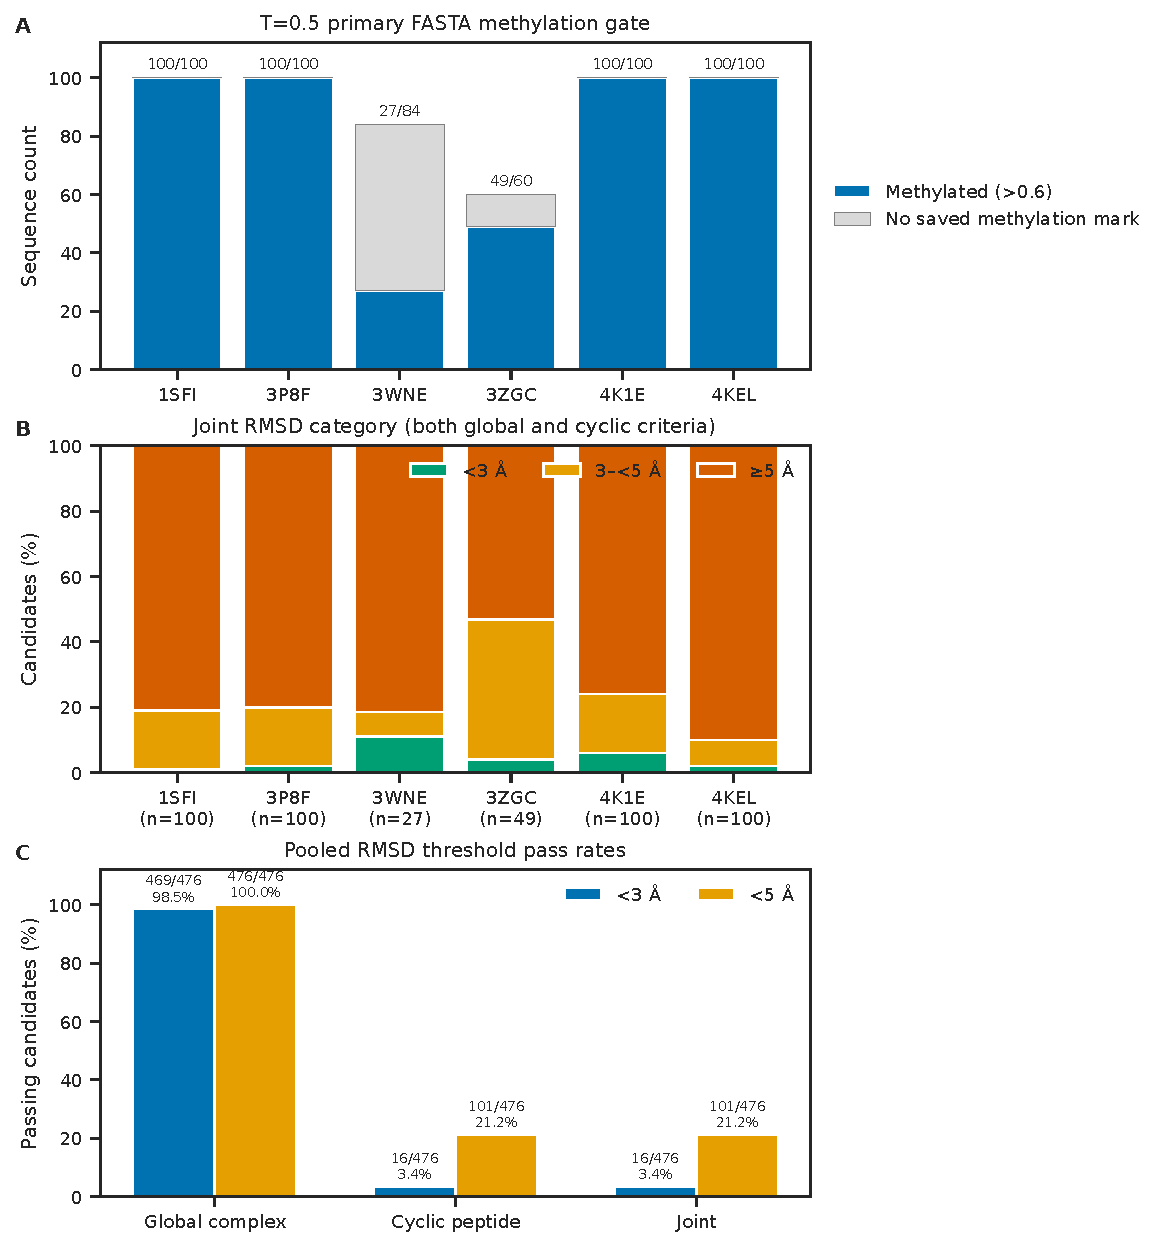
\includegraphics[width=0.98\textwidth]{figures/Fig1_cohort_and_rmsd_pass_rates.pdf}
  \caption{六个非3AV复合物的队列漏斗与RMSD通过率（Fig.~1）。
  （A）各靶点原始生成及严格$p>0.6$后保留数量；（B）各靶点联合RMSD类别；
  （C）总体全复合物、环肽以及二者联合的通过率。图中的结构通过率以476条
  保留设计为分母；从544条原始生成开始的端到端产率另见
  表~\ref{tab:six-raw-yield}。}
  \label{fig:task1-six-fig1}
\end{figure}

\subsection{RMSD分布与联合结构成功率}

按照预设口径，每个样本只进行一次全复合物CA叠合；随后在该坐标系内，对末链
环肽采用完整CA配对和最佳正向循环移位，不允许反向遍历，也不进行第二次肽链
单独拟合。联合通过要求同一条设计的全复合物CA RMSD与最佳正向循环肽CA RMSD
同时严格小于相应阈值。

在476条保留设计中，全复合物CA RMSD的总体中位数为
$1.022\,[0.692,1.534]~\angstrom$，最佳正向循环肽CA RMSD的总体中位数为
$6.738\,[5.261,8.129]~\angstrom$（中括号内为四分位距，表~\ref{tab:six-rmsd}）。
全复合物部分有$469/476=98.53\%$低于$3~\angstrom$，且$476/476=100\%$
低于$5~\angstrom$；因此总体失败主要由环肽在已经对齐的复合物坐标系中的
位置或构象偏差驱动，而不是受体整体叠合失败。

联合$<3~\angstrom$共有16条，保留后条件成功率为
$16/476=3.36\%$，95\% Wilson置信区间为$2.08\%$--$5.39\%$；联合
$<5~\angstrom$共有101条，条件成功率为$101/476=21.22\%$，95\% Wilson
置信区间为$17.78\%$--$25.11\%$。换用544条原始生成作分母时，对应端到端
产率分别为$2.94\%$（95\% Wilson置信区间$1.82\%$--$4.72\%$）和
$18.57\%$（$15.52\%$--$22.05\%$）。这两组数字不可互换：前者评价已生成
有效甲基化标记后的结构质量，后者回答一次原始生成最终得到合格设计的概率。

\begin{table}[H]
  \centering
  \caption{保留设计的RMSD分布与联合通过率}
  \label{tab:six-rmsd}
  \small
  \begin{adjustbox}{max width=\textwidth}
  \begin{tabular}{lrrrrr}
    \toprule
    靶点 & 保留数 &
    \makecell{全复合物CA RMSD\\中位数 [IQR]（\AA）} &
    \makecell{循环肽CA RMSD\\中位数 [IQR]（\AA）} &
    \makecell{联合$<3\,\angstrom$\\分子/保留数（\%）} &
    \makecell{联合$<5\,\angstrom$\\分子/保留数（\%）} \\
    \midrule
    1SFI & 100 & 0.884 [0.581, 1.457] & 6.289 [5.239, 7.814] & 1/100（1.00） & 19/100（19.00） \\
    3P8F & 100 & 0.981 [0.445, 1.364] & 6.375 [5.301, 7.282] & 2/100（2.00） & 20/100（20.00） \\
    3WNE & 27  & 0.904 [0.893, 0.927] & 29.002 [22.337, 39.916] & 3/27（11.11） & 5/27（18.52） \\
    3ZGC & 49  & 2.337 [1.662, 2.742] & 5.219 [4.367, 6.377] & 2/49（4.08） & 23/49（46.94） \\
    4K1E & 100 & 1.041 [0.691, 1.517] & 6.803 [5.071, 7.809] & 6/100（6.00） & 24/100（24.00） \\
    4KEL & 100 & 1.133 [0.701, 1.491] & 7.791 [6.361, 10.364] & 2/100（2.00） & 10/100（10.00） \\
    \midrule
    \textbf{总体} & \textbf{476} & \textbf{1.022 [0.692, 1.534]} &
    \textbf{6.738 [5.261, 8.129]} & \textbf{16/476（3.36）} &
    \textbf{101/476（21.22）} \\
    \bottomrule
  \end{tabular}
  \end{adjustbox}
  \par\vspace{2pt}
  \footnotesize 注：IQR为第25至第75百分位。表内百分比均以本靶点“保留数”为
  分母；总体$<3~\angstrom$与$<5~\angstrom$比例的95\% Wilson置信区间
  分别为$2.08\%$--$5.39\%$和$17.78\%$--$25.11\%$。
\end{table}

靶点层面的结果进一步说明为什么必须同时报告分子与分母。3WNE的环肽RMSD
中位数最高（$29.002~\angstrom$），但仍有$3/27$条低于$3~\angstrom$；由于其
仅保留27条，换成原始生成分母后为$3/84=3.57\%$。3ZGC的条件联合
$<5~\angstrom$比例最高（$23/49=46.94\%$），其端到端产率则为
$23/60=38.33\%$。这些描述性差异不应被解释为经多重比较校正后的靶点排名。
完整分布及两个RMSD之间的关系见图~\ref{fig:task1-six-fig2}。

\begin{figure}[p]
  \centering
  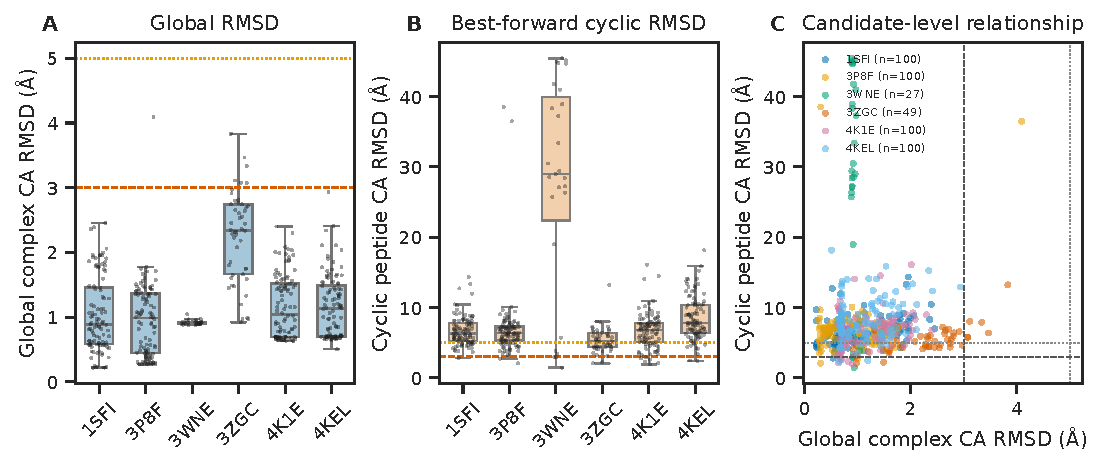
\includegraphics[width=0.98\textwidth]{figures/Fig2_rmsd_distributions.pdf}
  \caption{六个非3AV复合物的RMSD分布与关系（Fig.~2）。全复合物CA RMSD
  来自唯一一次全复合物叠合；循环肽CA RMSD在同一坐标系内采用最佳正向循环
  移位计算。虚线标示$3~\angstrom$与$5~\angstrom$阈值。}
  \label{fig:task1-six-fig2}
\end{figure}

作为表示方式敏感性分析，如果不允许循环移位而强制使用固定残基顺序，联合
$<3~\angstrom$和$<5~\angstrom$分别仅为$2/476=0.42\%$和
$33/476=6.93\%$；采用最佳正向循环移位后分别为$16/476=3.36\%$和
$101/476=21.22\%$。这一变化反映环状序列起点的表示等价性，并非重新生成或
重新拟合后的模型性能提升；主结果始终使用预先规定的最佳正向循环移位口径。

\subsection{甲基化输出的组成}

图~\ref{fig:task1-six-fig3}给出476条保留设计中甲基化位点和每条序列甲基化
数量的分布。这里的小写字母只是原始生成器在严格$p>0.6$规则下保存的预测
甲基化标记；它们不是实验测得的修饰状态，也不能据此推断真实酶学位点偏好。
该图的作用是描述进入RMSD分析的设计队列，而不是重新评价甲基化分类器的
独立准确率。

\begin{figure}[p]
  \centering
  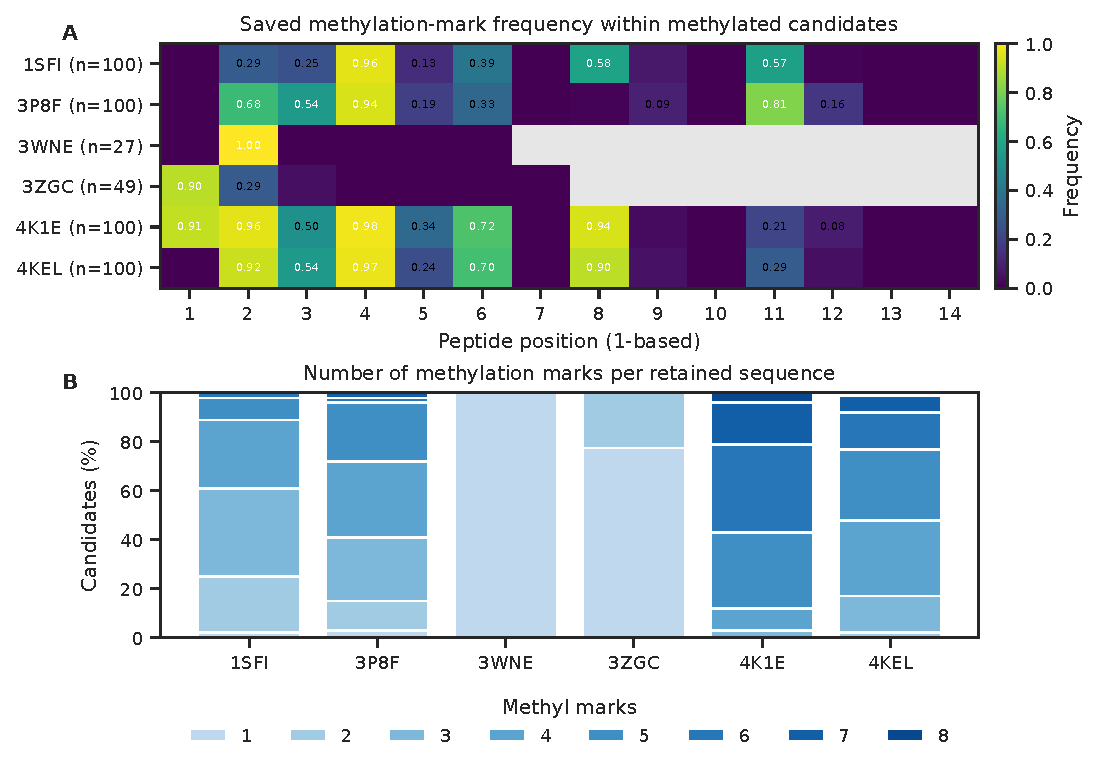
\includegraphics[width=0.98\textwidth]{figures/Fig3_methylation_positions_and_counts.pdf}
  \caption{保留设计的预测甲基化位置与数量（Fig.~3）。序列中的小写残基表示
  原始生成文件按严格$p>0.6$保存的甲基化预测；位点编号为设计肽链的1基坐标。}
  \label{fig:task1-six-fig3}
\end{figure}

\subsection{每靶点oracle代表与选择条件化的下游读数}

为便于逐个靶点查看具体序列，从每个靶点的保留设计中选取最佳正向循环肽CA
RMSD最小的一条，得到六条oracle代表（表~\ref{tab:six-oracle}）。六条代表的
循环肽RMSD均低于$3~\angstrom$，但这一事实是选择规则的直接结果，不能代替
随机或预先固定候选上的成功率估计。图~\ref{fig:task1-six-fig5}汇总这些代表的
RMSD、预测通透性、固定构象PyRosetta界面能以及结构文件CA B-factor均值代理量。

\begin{table}[H]
  \centering
  \caption{六个靶点按最小循环肽RMSD选择的oracle代表}
  \label{tab:six-oracle}
  \scriptsize
  \begin{adjustbox}{max width=\textwidth}
  \begin{tabular}{llrrrrrr}
    \toprule
    靶点 & 设计序列 & 甲基化位点 &
    \makecell{全复合物\\RMSD（\AA）} &
    \makecell{循环肽\\RMSD（\AA）} &
    \makecell{预测通透性\\（模型单位）} &
    \makecell{固定构象\\界面能（REU）} &
    \makecell{CA B-factor\\均值代理量} \\
    \midrule
    1SFI & \seq{RCCrGNCGQCQFGG} & 4 & 0.536 & 2.818 & $0.454$ & 31.77 & 93.49 \\
    3P8F & \seq{CrrrGrQGKGrRGC} & 2,3,4,6,11 & 0.300 & 2.075 & $7.57\times10^{-35}$ & $-25.73$ & 91.57 \\
    3WNE & \seq{GrKWNC} & 2 & 0.933 & 1.459 & $0.0864$ & 0.73 & 90.03 \\
    3ZGC & \seq{rEGGQNR} & 1 & 0.973 & 2.076 & $1.04\times10^{-7}$ & 15.95 & 89.91 \\
    4K1E & \seq{rcrrrQCrQGNCDR} & 1,2,3,4,5,8 & 0.900 & 1.916 & $6.14\times10^{-32}$ & 434.24 & 89.04 \\
    4KEL & \seq{RcrrGNCrQGFCDR} & 2,3,4,8 & 0.655 & 2.379 & $0.00214$ & 416.77 & 91.49 \\
    \bottomrule
  \end{tabular}
  \end{adjustbox}
  \par\vspace{2pt}
  \footnotesize 注：每行均在观察该靶点全部候选的循环肽RMSD后再选择，故所有
  后续读数均为选择条件化描述。CA B-factor均值只是相应结构文件字段的代理量，
  不应与来自另一流程、另一标定方式的pLDDT直接等同。通透性列没有实验标签，
  也没有校准到物理单位。
\end{table}

\begin{tcolorbox}[colback=SoftAmber,colframe=Amber,title={oracle选择警告}]
表~\ref{tab:six-oracle}中的序列并非预先指定，也不是从476条设计中随机抽取；
它们是在观察目标结局——循环肽RMSD——之后逐靶点取最小值。因此，代表序列
及图~\ref{fig:task1-six-fig5}中的下游指标只能用于候选展示和后续验证优先级，
不能用于估计模型的总体成功概率，也不能把六条代表的均值当作未选择队列的
无偏性能。通透性预测同样是在该选择之后报告，应视为探索性结果。固定构象
PyRosetta界面能未经过统一松弛或重打包，而结构文件中的
\path{highfold_ca_bfactor_mean}仅作置信度代理；二者均不构成实验结合或稳定性
证据。无选择偏倚的成功率应以表~\ref{tab:six-raw-yield}和
表~\ref{tab:six-rmsd}中的全部544条或476条记录为准。
\end{tcolorbox}

\begin{figure}[p]
  \centering
  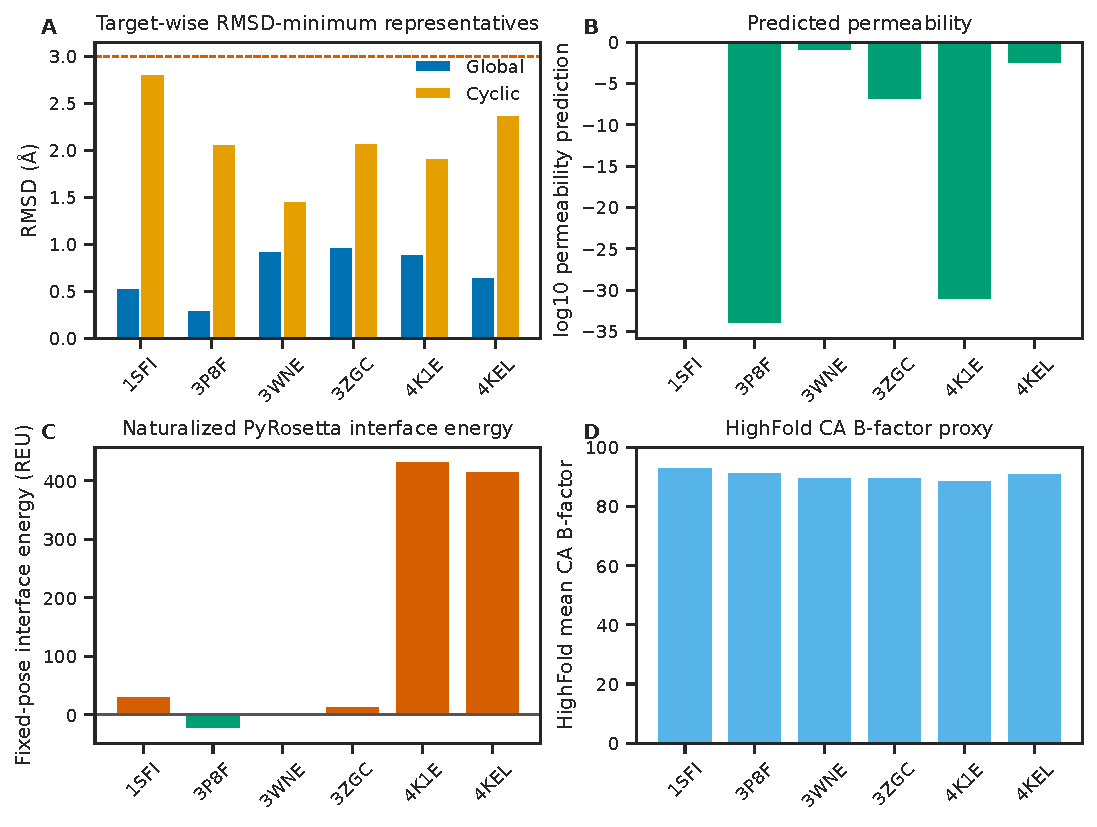
\includegraphics[width=0.98\textwidth]{figures/Fig5_selection_conditioned_downstream_metrics.pdf}
  \caption{六条oracle代表的选择条件化下游指标（Fig.~5）。（A）全复合物与
  循环肽RMSD；（B）预测通透性（log10尺度）；（C）固定构象PyRosetta界面能；（D）结构
  文件CA B-factor均值代理量。所有面板均须结合正文的oracle选择警告解释。}
  \label{fig:task1-six-fig5}
\end{figure}
